\subsection{Linear mode without matches}\label{app:no-matches}

States are penalized by the number of remaining seeds that cannot be matched. So,
curiously, matches are not always needed to direct the \A search to an optimal path. In
fact, when each seed contains exactly one mutation \sh scales linearly even though
there are no matches, as shown by the artificial example in
\cref{fig:no-matches}.

\begin{figure}[h]
  \centering
  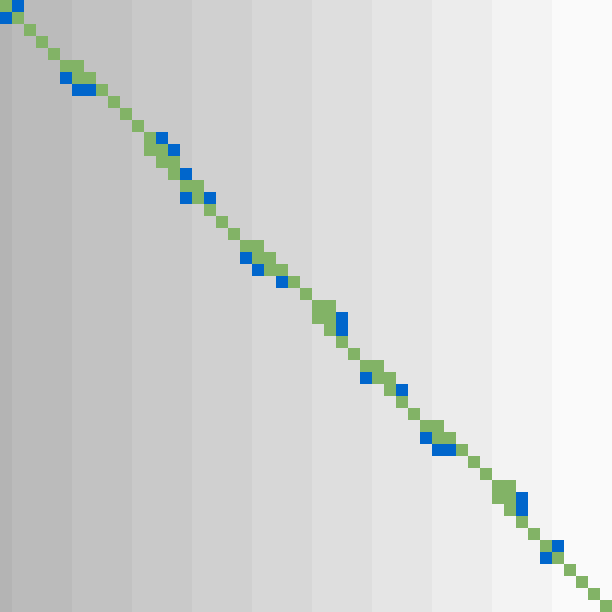
\includegraphics[width=0.7\linewidth]{imgs/no-matches.png}
  \caption[Artificial example of \A with \sh with no matches]{\textbf{Artificial example of \A with \sh with no matches}
  ($n{=}m{=}50$, $r{=}1$, $k{=}5$, $80\%$ similarity, $1$ mutation per seed alternating
  substitution, insertion, and deletion). The background colour indicates
  $\hsh(u)$ with higher values darker. Expanded states are
  green~(\greensquare{}), open states blue~(\bluesquare{}).}
  \label{fig:no-matches}
\end{figure}
